\documentclass[11pt]{article}
\usepackage{fontspec}
\setmainfont{Times New Roman}
\usepackage{amsmath,amssymb}
\usepackage[margin=2.3cm]{geometry}
\usepackage{booktabs,graphicx,xcolor}
\usepackage{hyperref}
\hypersetup{colorlinks=true,urlcolor=blue}
\sloppy

\hypersetup{pdftitle={Uniformly accelerated rectilinear motion},pdfsubject={PhysLab study guide, content canonical v2 (7d85de57), lang en},pdfauthor={PhysLab},pdflang={en}}
\begin{document}
{\small\color{gray} PhysLab / ЕНТ • ҰБТ / English \quad study guide v2 \quad content canonical v2 (7d85de57)}

\section*{Uniformly accelerated rectilinear motion}
\subsection*{Goal}
After the video the student can find the velocity and displacement of a uniformly accelerated body from initial velocity, acceleration and time, and check the answer by the area under the v(t) graph.

\subsection*{The idea in brief}
If speed never changes, motion is uniform: v equals s over t.

Here speed grows — but grows by the same amount each second.

Every second adds three metres per second — that is what an acceleration of three means.

Such motion is called uniformly accelerated.

Acceleration measures how fast velocity grows: a equals the change in velocity divided by time.

Its unit is the metre per second squared.

We point the x axis along the motion: everything forward takes the plus sign.

Velocity at any moment is the starting velocity plus the gain.

The gain is acceleration times time: v equals v naught plus a t.

Check the units: metres per second squared times seconds gives metres per second.

Displacement is how far the body shifted from the start.

While direction stays the same, it equals the distance travelled.

The slope of the line is the acceleration: the steeper, the larger the a.

Remember: the slope of the v–t graph equals the acceleration.

The area under the velocity graph numerically equals the displacement.

\subsection*{Quantities and units}
\begin{tabular}{lll}\toprule
$v_0$ & initial velocity & 2 m/s \\
$a$ & acceleration & 3 m/s² \\
$t$ & time & 4 s \\
$v$ & final velocity & 14 m/s \\
$s$ & displacement & 32 m \\
\bottomrule\end{tabular}

\subsection*{Formulas and conditions}
\textbf{Definition of acceleration:} \[a = \Delta v / \Delta t\]
\textbf{Velocity:} \[v = v_0 + at\]
\textbf{Displacement:} \[s = v_0 t + at^2/2\]
\textbf{Displacement via average velocity:} \[s = (v_0 + v)t/2\]
\begin{itemize}
\item Motion is rectilinear, the x axis points along the motion.
\item Acceleration is constant in magnitude and direction.
\item Velocity keeps its sign — no reversal, displacement equals distance.
\item All quantities in SI: m, s, m/s, m/s².
\end{itemize}

\subsection*{Figures}
\begin{figure}[htbp]\centering
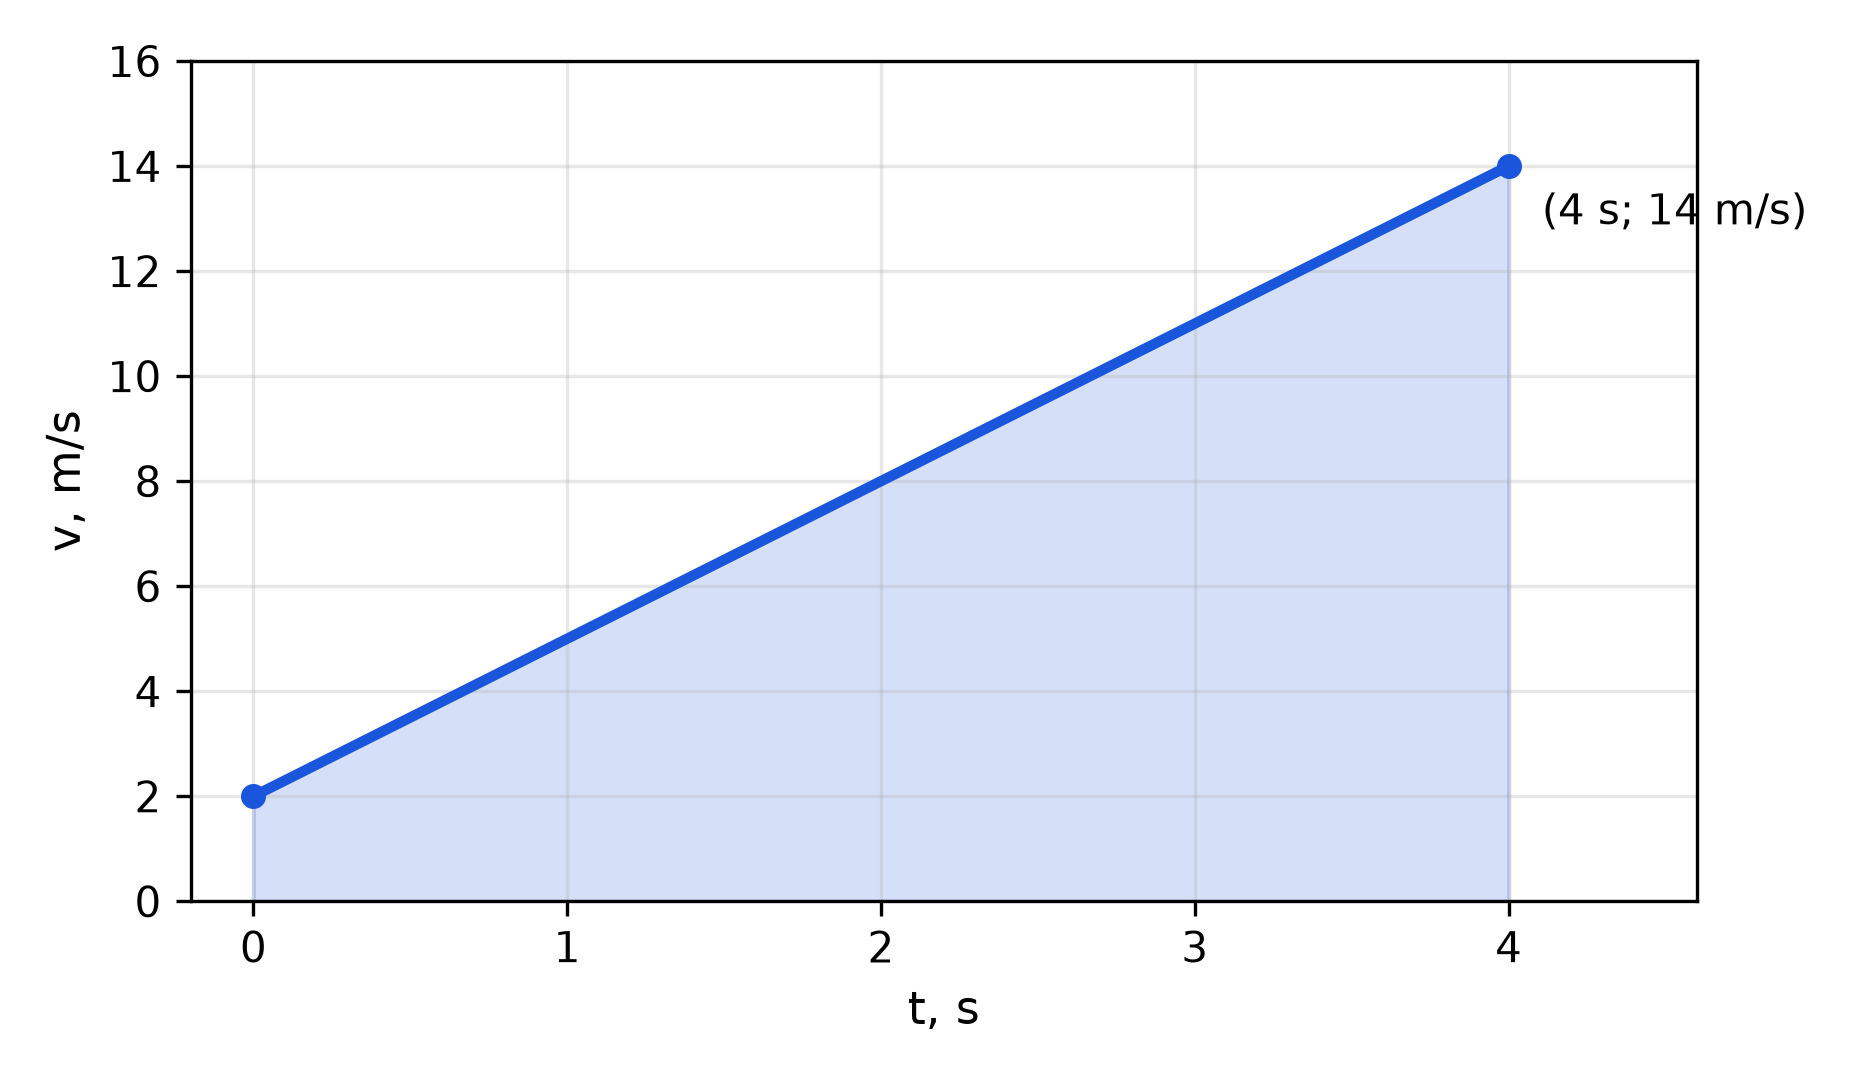
\includegraphics[width=0.85\textwidth]{fig_vt_en.png}\caption{Graph of $v(t) = 2 + 3t$: the slope is the acceleration $a = 3$; the shaded area is the displacement $s = 32$.}\end{figure}

\begin{figure}[htbp]\centering
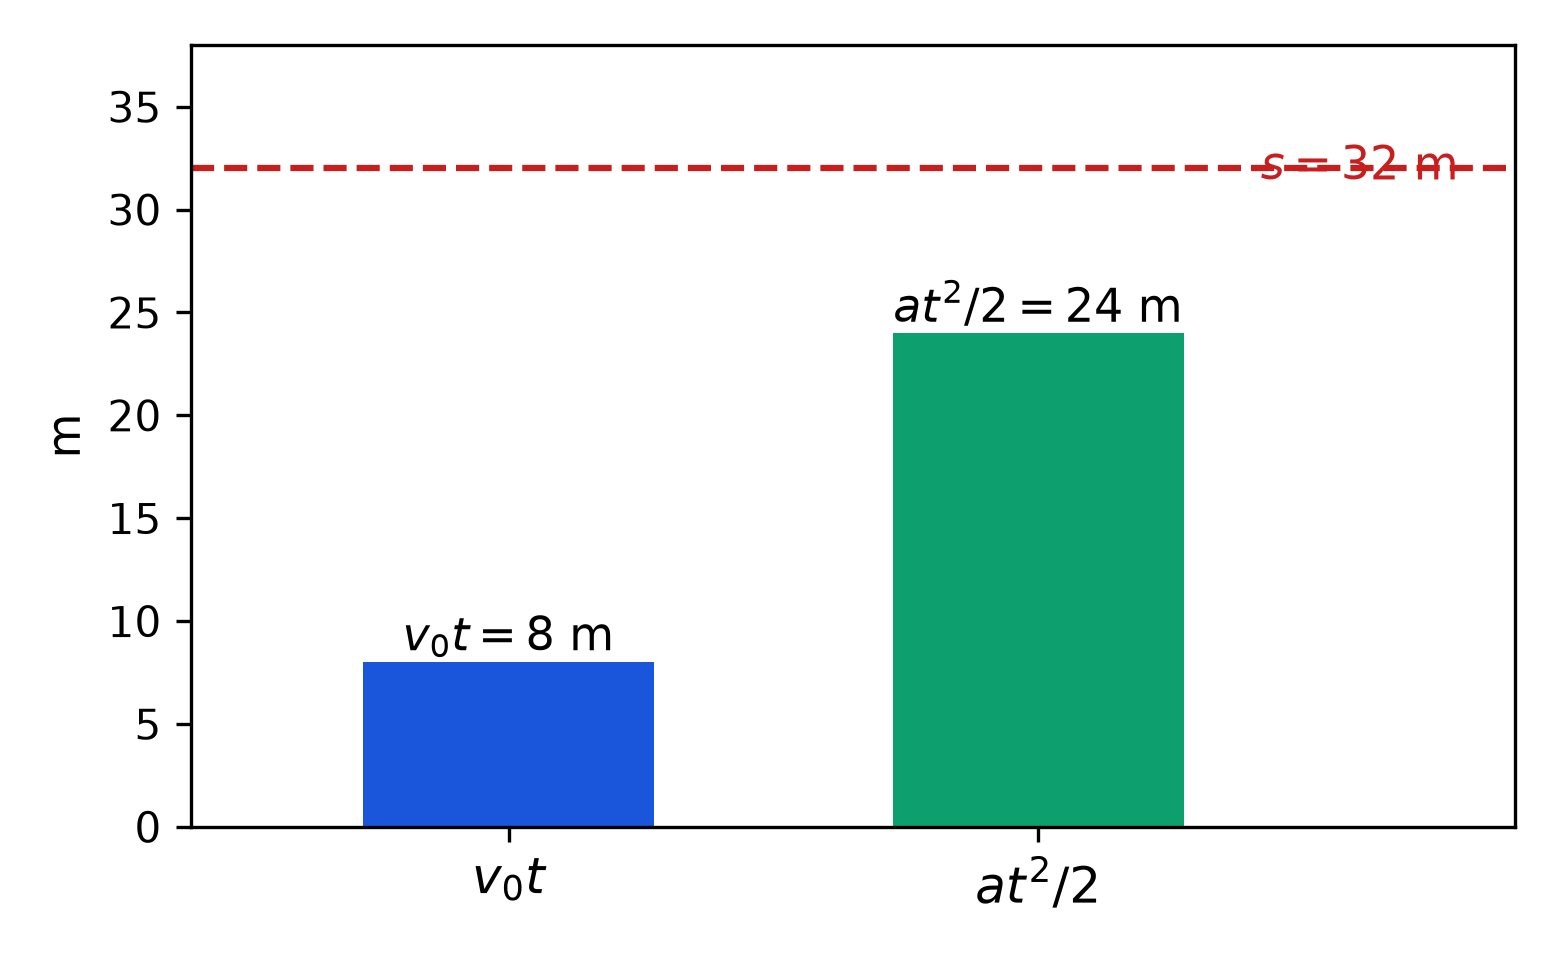
\includegraphics[width=0.7\textwidth]{fig_bars_en.png}\caption{Displacement in two terms: $v_0t = 8$ plus $at^2/2 = 24$; total $s = 32$ m.}\end{figure}

\subsection*{Worked example}
Given: $v_0 = 2$ m/s, $a = 3$ m/s², $t = 4$ s. Find: $v$, $s$.

\begin{enumerate}
\item $v = v_0 + at = 2 + 3\cdot 4 = 14$ m/s.
\item $s = v_0t + at^2/2 = 2\cdot 4 + 3\cdot 16/2 = 8 + 24 = 32$ m.
\item $s = (v_0+v)t/2 = (2+14)\cdot 4/2 = 32$ m.
\end{enumerate}
Units check: m/s² · s = m/s — consistent.

\subsection*{Traps}
\begin{itemize}
\item Trap 1: $14\cdot 4 = 56$ — wrong: the speed was growing, take the average.
\item Trap 2: slope is acceleration, area is displacement.
\end{itemize}

\subsection*{Practice tasks}
\begin{enumerate}
\item An object starts at 2 m/s and accelerates at 3 m/s². What is its speed after 4 seconds?
\textbf{A)} 14 m/s \quad \textbf{B)} 12 m/s \quad \textbf{C)} 9 m/s \quad \textbf{D)} 6 m/s

\item An object moves with initial speed 2 m/s and acceleration 3 m/s² without changing direction. Find its displacement in 4 s.
\textbf{A)} 32 m \quad \textbf{B)} 56 m \quad \textbf{C)} 24 m \quad \textbf{D)} 20 m

\item Which motion is called uniformly accelerated?
\textbf{A)} Velocity changes by equal amounts in equal times \quad \textbf{B)} Velocity stays constant \quad \textbf{C)} Acceleration changes over time \quad \textbf{D)} Distance is the same in equal times

\item What does the slope of the line on a velocity–time graph show?
\textbf{A)} Acceleration \quad \textbf{B)} Displacement \quad \textbf{C)} Velocity \quad \textbf{D)} Time

\item On a v(t) graph a straight line runs from (0 s; 2 m/s) to (4 s; 14 m/s). Find the displacement.
\textbf{A)} 32 m \quad \textbf{B)} 48 m \quad \textbf{C)} 56 m \quad \textbf{D)} 24 m

\item A car starts from rest with acceleration 2 m/s². How far does it go in 5 s?
\end{enumerate}
\newpage\subsection*{Answers}
\begin{enumerate}
\item \textbf{A} — Acceleration adds 3 m/s of speed each second. So $v = v_0 + at = 2 + 3\cdot 4 = 14$ m/s.

\item \textbf{A} — $s = v_0t + at^2/2 = 2\cdot 4 + 3\cdot 16/2 = 8 + 24 = 32$ m. 56 m comes from plugging the final speed into the uniform-motion formula.

\item \textbf{A} — In uniformly accelerated motion velocity gains equal increments in equal times while acceleration stays constant (Zakirova 9, §3). D describes uniform motion.

\item \textbf{A} — The slope of v(t) equals acceleration: $a = \Delta v/\Delta t$. Displacement is the area under the graph, not the slope (Zakirova 10, §3).

\item \textbf{A} — Trapezoid area: $(2 + 14)/2 \cdot 4 = 32$ m. 24 m is the triangle alone, without the rectangle.

\item \textbf{25 m} — $s = 0\cdot 5 + 2\cdot 25/2 = 25$ m.
\end{enumerate}

\subsection*{Sources}
Definitions, formulas and graph rules are cross-checked against the textbooks; numbers are PDF page numbers. Guide tasks are original.
\begin{itemize}
\item Физика Закирова 9.pdf — definitions and formula table: PDF с. 19–29.
\item Физика Закирова 10 ЖМ.pdf — graphs and the area rule (§3): PDF с. 15–18, 20.
\item FBS (1).pdf — formula and term cross-check (Sailaubaev): PDF с. 6–7.
\item Testcenter -3.pdf — ENT graph-area task format (task 1, p. 2; key B, p. 37): PDF с. 2, 37.
\item NCT physics sample (ru): \url{https://new.testcenter.kz/wp-content/uploads/2024/12/obr_var_test_02.pdf}
\item NCT physics sample (en): \url{https://new.testcenter.kz/wp-content/uploads/2025/06/PHYSICS.pdf}
\end{itemize}

Status: physics and keys independently checked (Stage G); translations and terms need teacher review.
\end{document}
